\section{Results}
\label{sec:results}

In the following sections, we explore the response of the log-loss and Brier score metrics to the prevalence of classifier error properties and as a function of the weighting scheme on the class(es) affected by each systematic.
Both of our metrics are strictly nonnegative and vanish for a truly perfect classifier.

\subsection{Mock classifier systematics}
\label{sec:mockresults}

We simulate mock classifications from linear combinations of the confusion matrices of Section~\ref{sec:mockdata} using a log-normal distribution of class populations to make a catalog of $10^{5}$ posterior probability vectors for every test case.
The limited catalog size induces a small amount of stochasticity, particularly due to the classes with only a handful of members.
% TODO: repeat for error bars

In Figure~\ref{fig:cruise}, we illustrate the effect on the metrics of adding to an initially perfect classifier each of four error properties:
uncertainty (lower left panel, described in Section~\ref{sec:uncertaindata}),
a class $\tilde{m}$ subsuming class $m'$ (upper right panel, described in Section~\ref{sec:inaccuratedata}),
and reducing perfection via uniform noise by a factor of $s=2$ to an almost perfect classifier and $s=4$ to a noisy classifier (upper left and bottom right panels, respectively, described in Section~\ref{sec:accuratedata}).
Flat weights are used for each of these tests.

\begin{figure}
	\begin{center}
		\label{fig:cruise}
		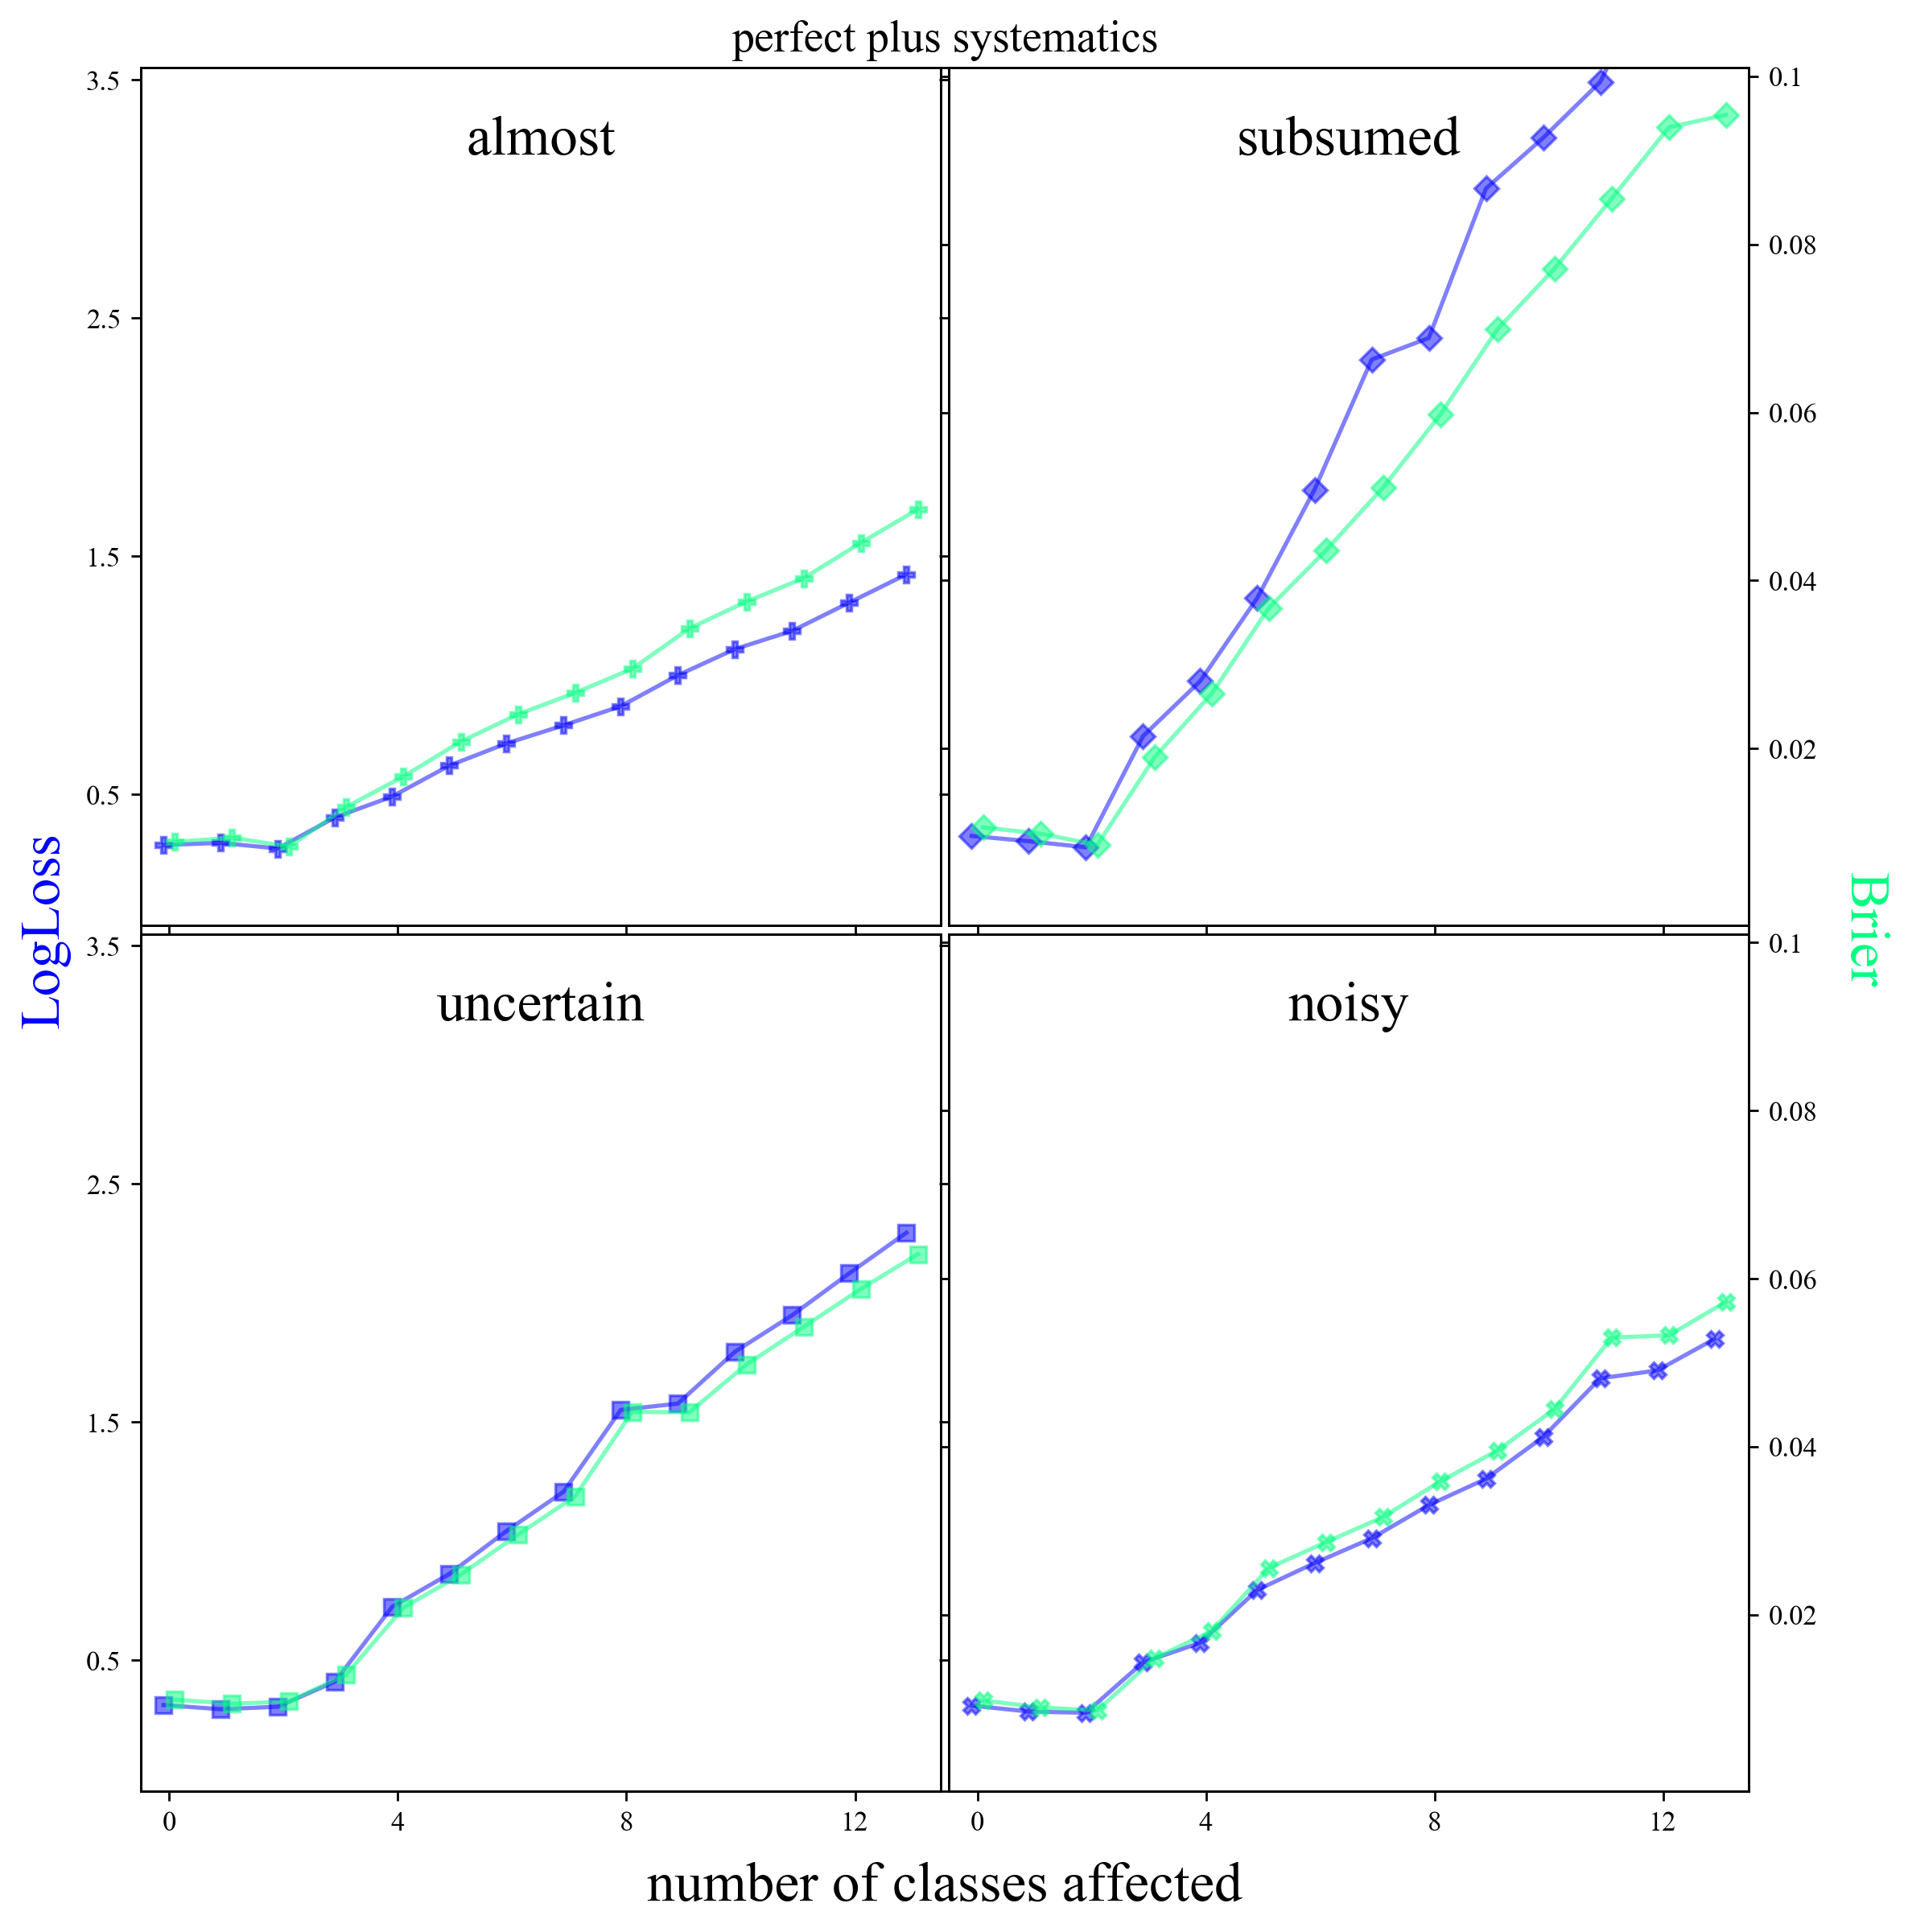
\includegraphics[width=0.5\textwidth]{./fig/systematics_onlyperfect.png}
		\caption{Systematic effects added to the perfect classifier.
		The log-loss and Brier scores (left and right $y$ axes, respectively) are shown for classifiers that are ``perfect'' aside from the indicated systematic (panels) as a function how many classes are affected by the systematic (on the $x$-axis), beginning with the lowest population classes.
		The two metrics behave very similarly to one another and have high sensitivity to a subsuming classifier.}
	\end{center}
\end{figure}

The roughly constant slopes of the metric values as a function of the number of classes affected by the systematics indicates that both the log-loss and Brier score are stable to the prevalence of each systematic.
The peak value of the metric when every class is thoroughly affected by a sytematic is also consistent with our intuitive ranking of how badly the classifiers should be penalized for each systematic; the subsuming classifier is penalized more than the uncertain classifier, the uncertain classifier is penalized more than the noisy classifier, and the noisy classifier is penalized more than the almost perfect classifier.

Both the log-loss and Brier score are appropriate for singling out a classifier that enables any class to subsume other classes, thereby confirming that the cruise control classifier will not in general outscore a classifier that avoids subsuming.
The log-loss is somewhat more sensitive to subsuming classification rates than the Brier score, but they otherwise have very similar sensitivity.

The flat weighting scheme of Figure~\ref{fig:cruise} means there is a one-to-one correspondence between the number of classes affected and the weights on affected and unaffected classes.
From this perspective, we may view the $x$ axis as also representing increasing weight on the affected systematic.
The perfect classifier with a systematic applied to only one class (or a few) is equivalent to the tunnel vision classifier applied to that systematic as a baseline.
Thus Figure~\ref{fig:cruise} also shows the effect of decreasing the weight on the a tunnel vision classifier as the $x$ coordinate increases, relative to a baseline of the systematics indicated in each panel.
The approximately linear relationship between metric value and fractional weight for tunnel vision classifier for each of the uncertain, almost perfect, and noisy baselines is to be expected, because the only weighting scheme we considered is linear.
However the slopes differ for each systematic.

Consider a weighting of $\sim0.8$ for a class affected by tunnel vision, leaving $\sim0.2$ to be shared evenly among all other classes uniformly affected by the other systematics.
Qualitatively, we would say that a classifier that is almost perfect for other classes is superior to one that is noisy, and a classifier that is noisy for other classes is still superior to one that is uniform; furthermore, the subsuming classifier is even more harshly penalized in this situation than the uncertain classifier, meaning both metrics are  consistent with our basic tests of intuition in this case.
However, this observation also indicates that the tunnel vision systematic is difficult to penalize, and that if the affected class is given a large weight, it can easily dominate the metric.
If all classes are of scientific importance, heavily unequal weighting can incentivize tunnel vision classification.

% We introduced weighting of per-class metrics to discourage `tunnel vision' and `cruise control' classifiers that can ignore classes other than the most common and nonetheless perform well by a metric.
Figure~\ref{fig:popweight} shows the impact of weighting the per-class metrics by the number of objects in the class as each is affected by one of the systematics and the other classes are held at the more realistic almost perfect performance.
The points show different classification schemes, and all points are coloured by the change in the weighting, dependent on the size of the population class being classified.
Conversely, the cruise control classifier and, to a lesser degree the noisy classifier, always has high log-loss and Brier score values regardless of the weight on the affected class.

\begin{figure}
	\begin{center}
		\label{fig:popweight}
		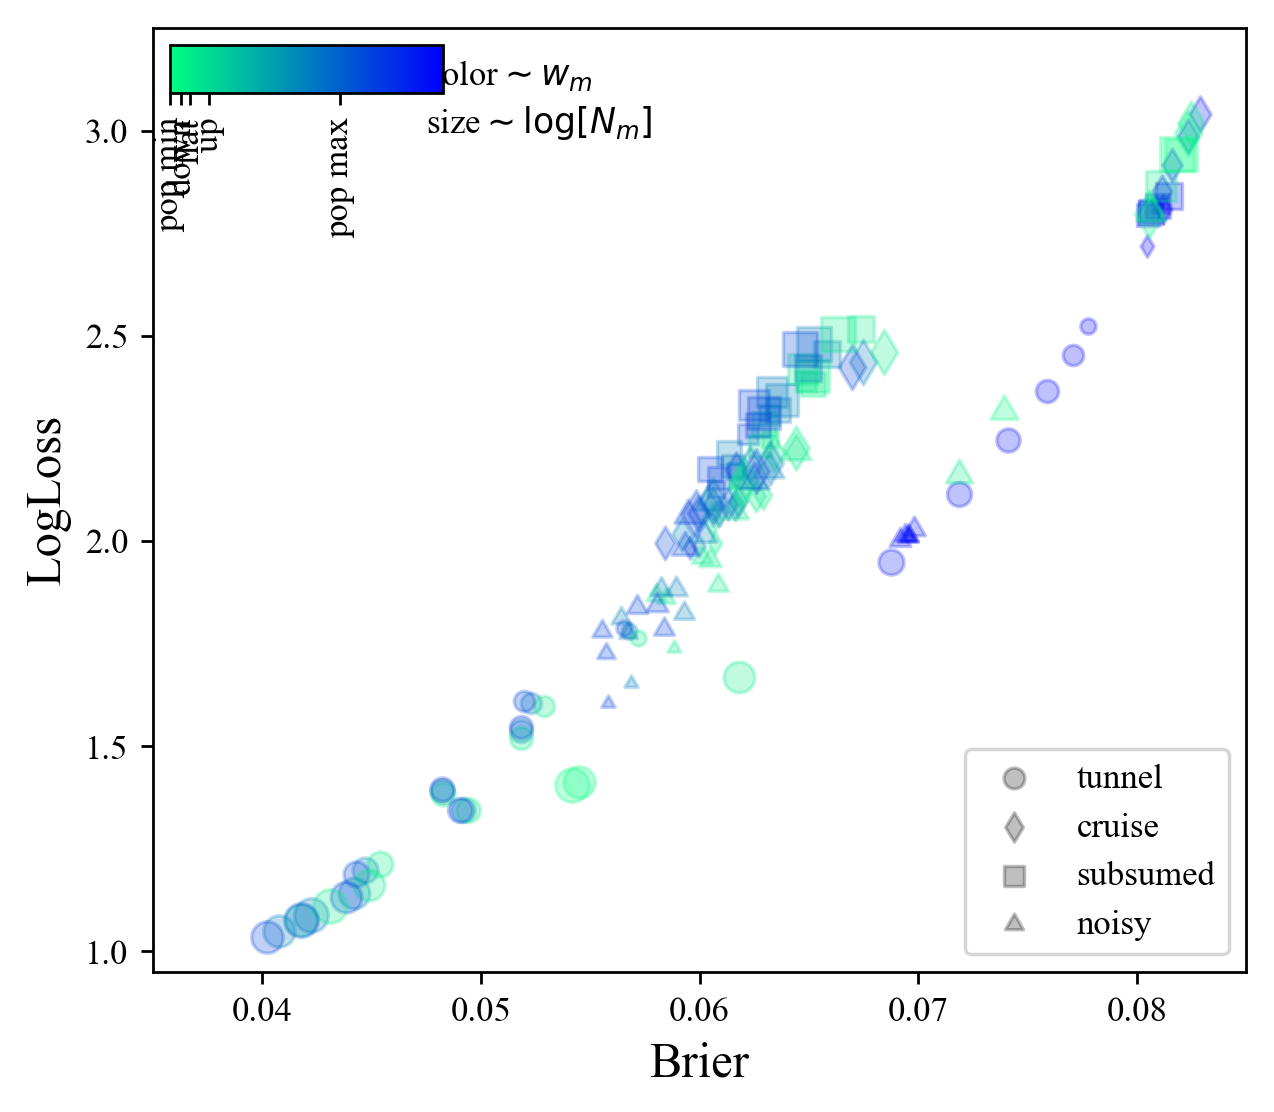
\includegraphics[width=0.5\textwidth]{./fig/all_effects_isolated.png}
		\caption{Population-weighted log-loss and Brier scores for classifiers with one class affected by a systematic, as a function of the population of the affected class.
		Each point corresponds to an almost perfect classifier that with one class instead affected by a systematic (shape).
		The metrics are calculated with a weighting (color and size) proportional to the log of its weight in a weighted average following Equation~\ref{eq:weightavg}.
		}
	\end{center}
\end{figure}

The tunnel vision classifier has a consistently low value under the Brier score and log-loss metric (bottom left corner of the plot), only increasing its Brier score once the weighting drops (less blue).
In this view, the Brier score appears to be more susceptible to tunnel vision than the log-loss, demonstrating a more significant decrease as the size of the affected class increases, but both metrics have concerning behavior in this regard.
This finding suggests that weighting alone may not be sufficient to counter the influence of this effect, and indicates a need for another balancing mechanism, such as requiring athreshold metric value on all classes.
% When considering a method of converting from one of these metrics to a finall `winner' of the classification challenge, care must be taken to ensure that all approaches do reasonably well at classifying more than one object.
% This thresholding procedure is discussed in the text

% \textbf{Ashish to reaplce/add more here?}
%\aim{Preliminary results indicate weighting will be very important for preventing the tunnel vision classifier from winning. It may be necessary to a priori anticipate which classes will have to be most strongly protected from this systematic via upweighting them.}

%\begin{figure}
%	\begin{center}
%		% 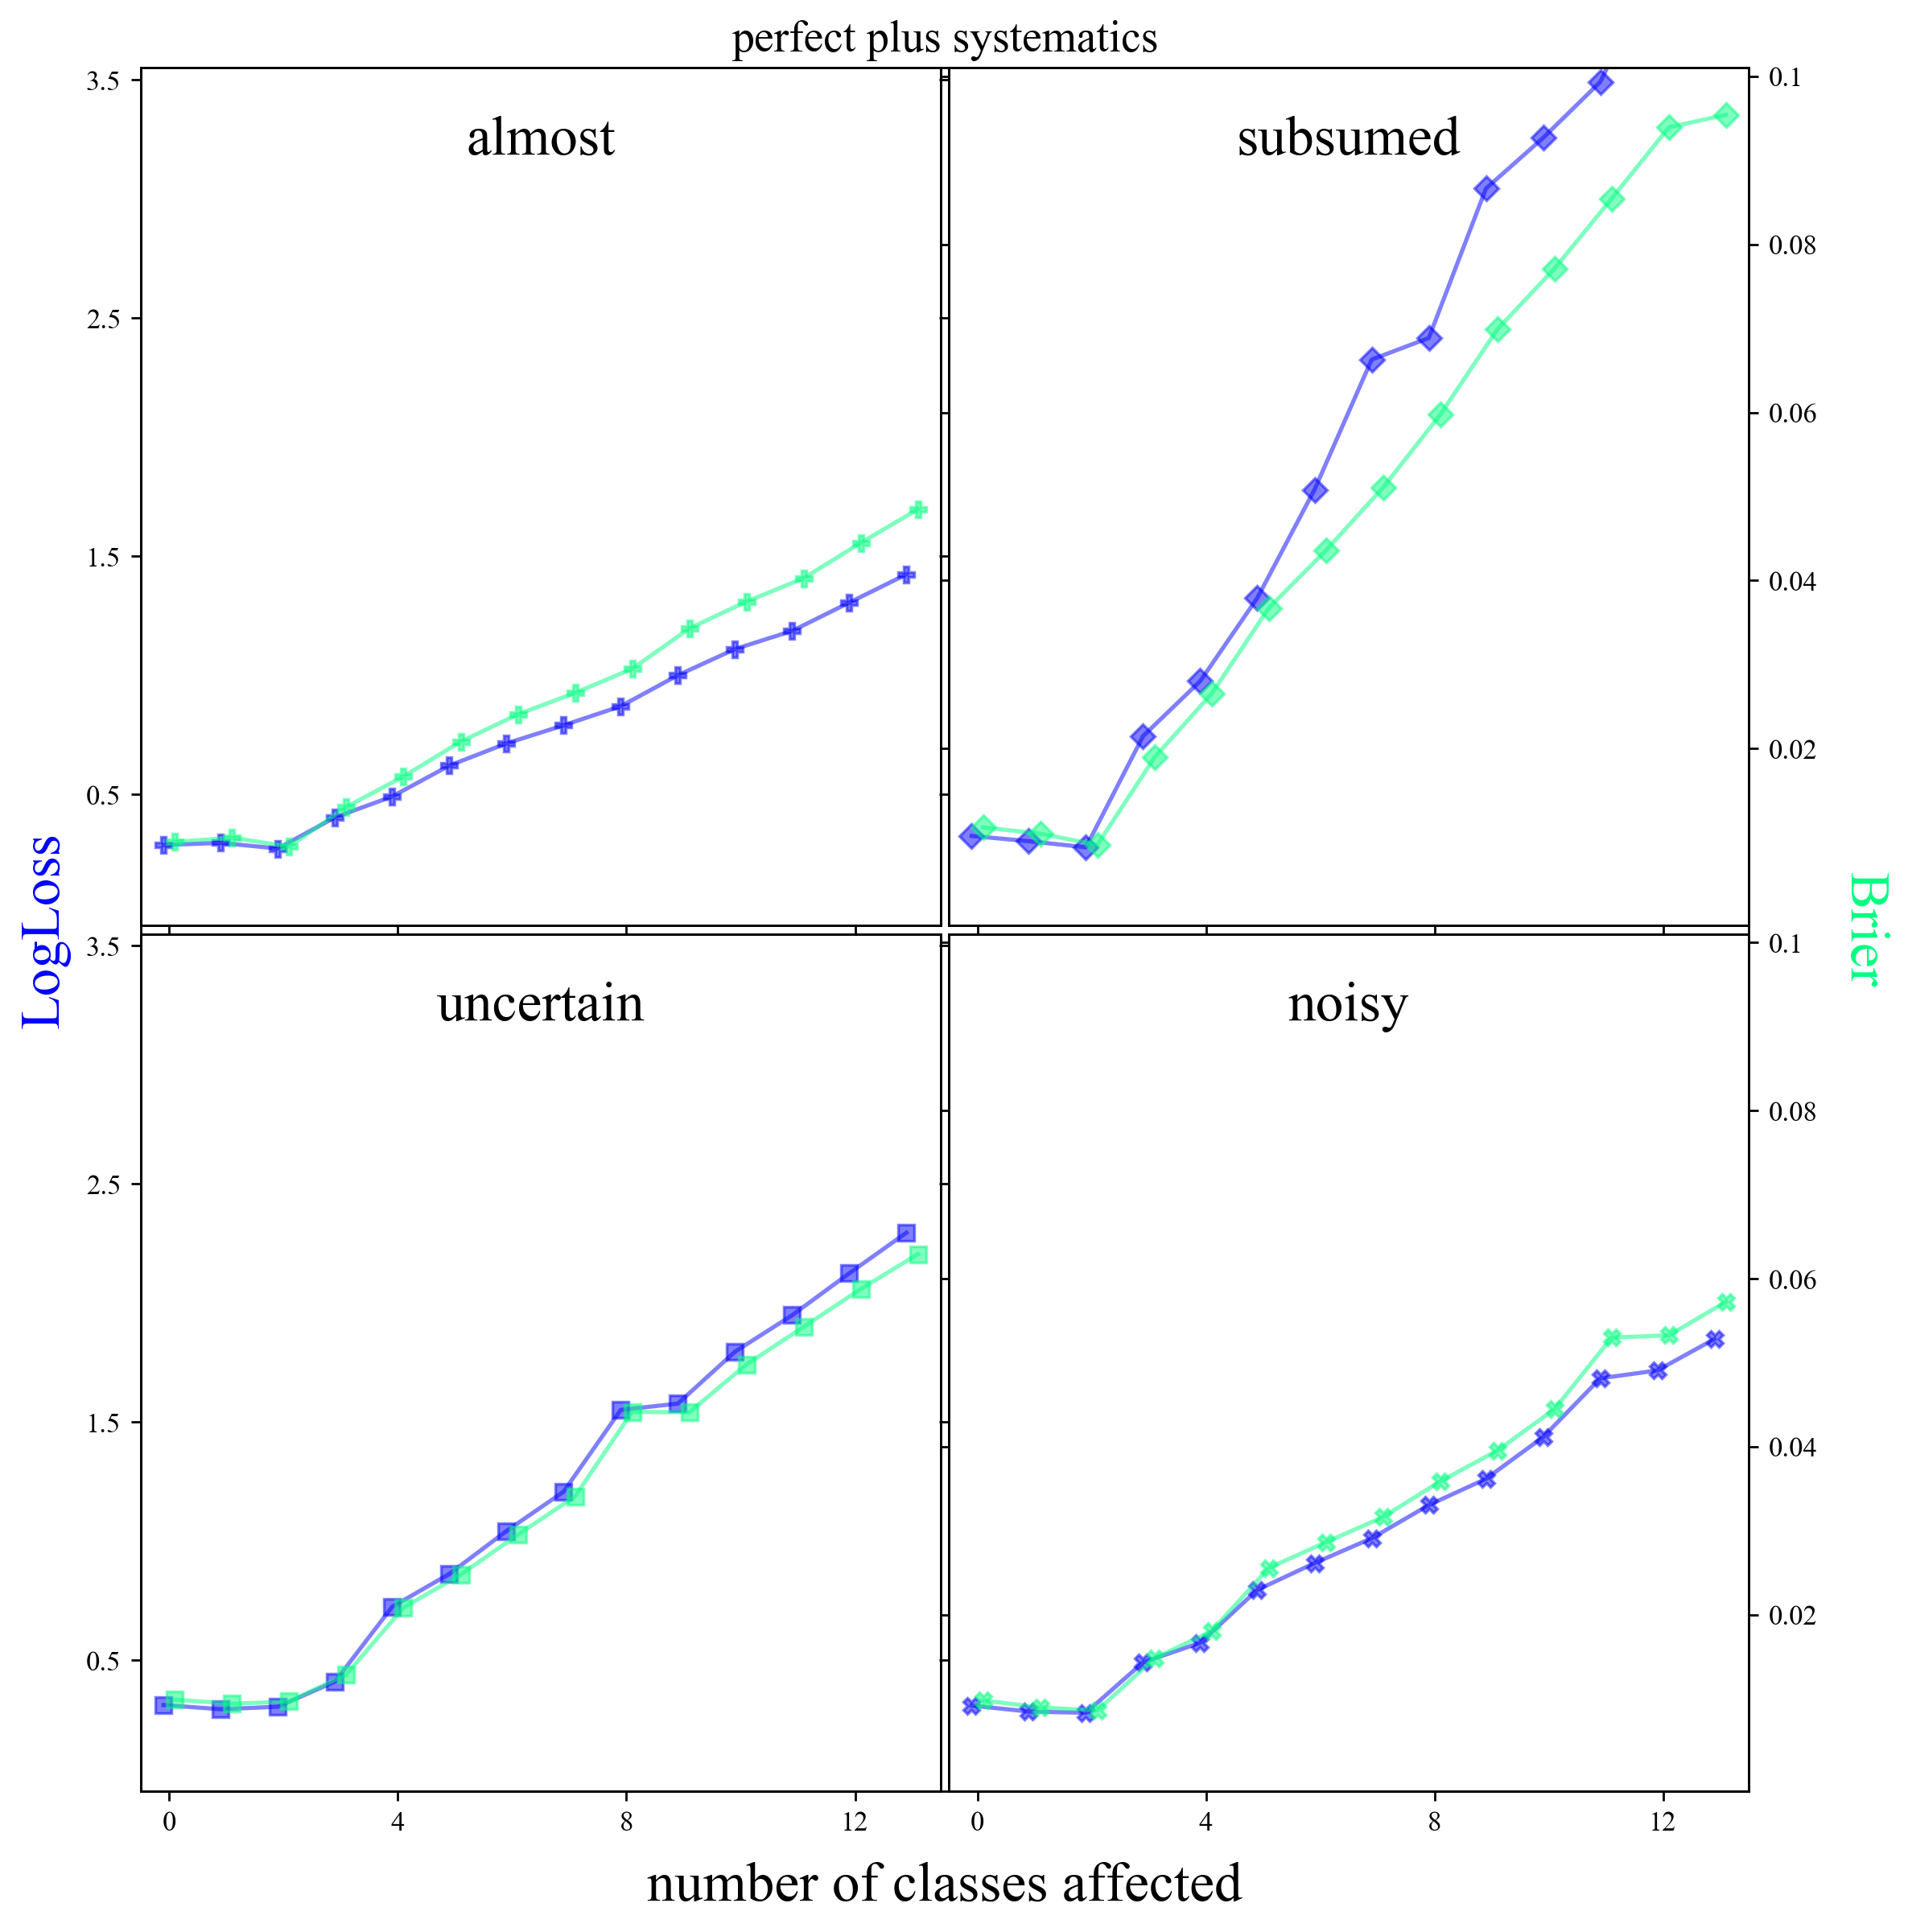
\includegraphics[width=0.5\textwidth]{./fig/systematics_onlyperfect.png}
%		\caption{\aim{After much iteration on how best to present these tests, a figure similar to Figure~\ref{fig:cruise} but for the tunnel vision classifier (heading) on different baseline classifications (panels) as a function of weight on the affected class (rather than number of classes) is under construction.}}
%		\label{fig:tunnel}
%	\end{center}
%\end{figure}

\subsection{Representative classifications}
\label{sec:realresults}

\begin{figure*}
	\begin{center}
		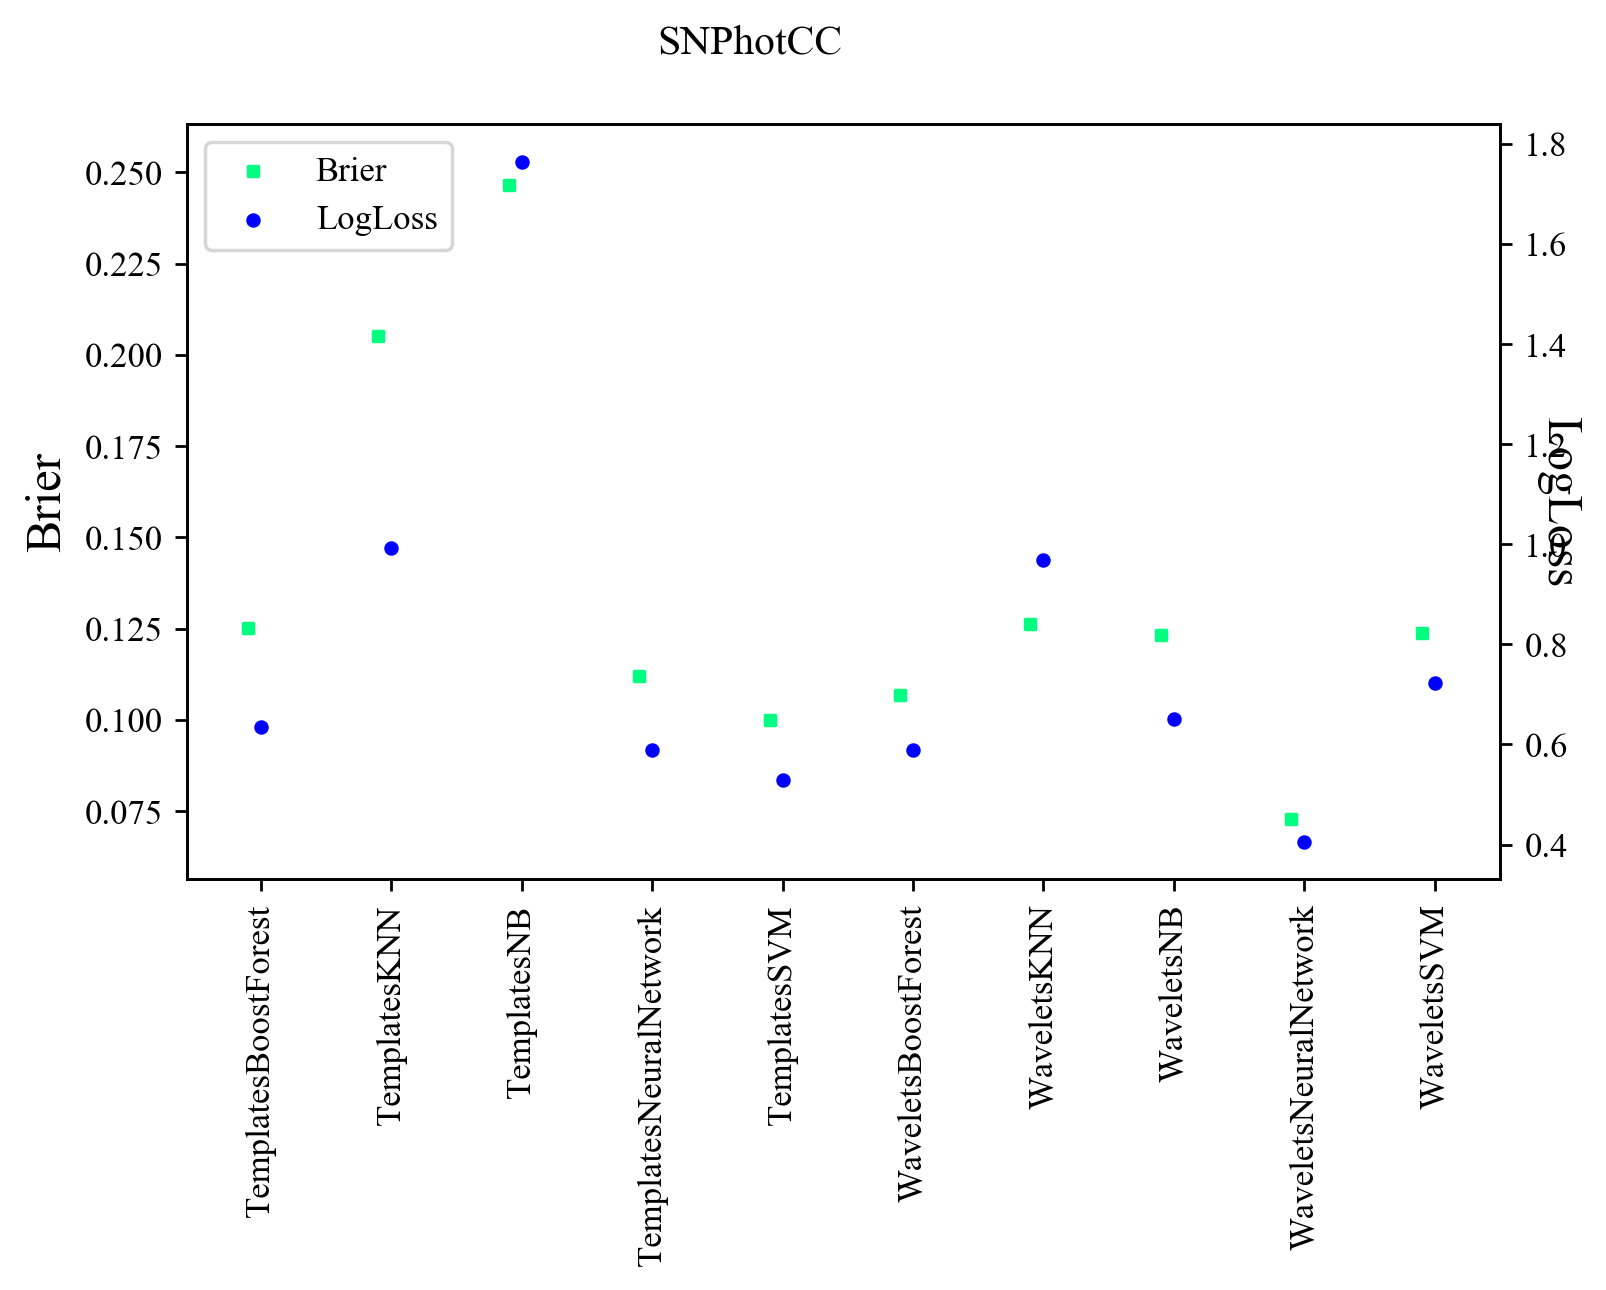
\includegraphics[width=0.85\textwidth]{./fig/SNPhotCC_res.png}\\
		 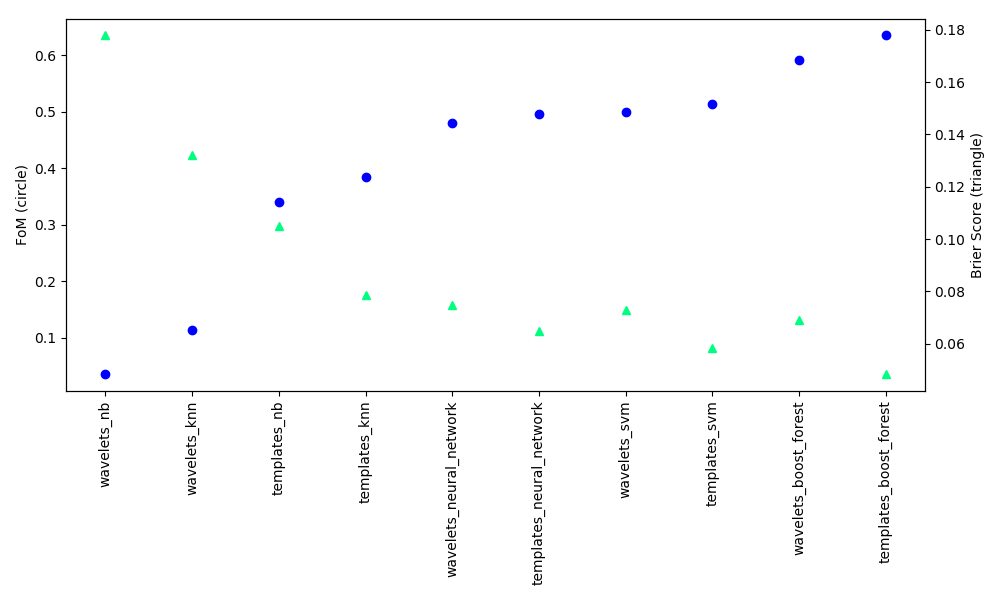
\includegraphics[width=0.8\textwidth]{./fig/fom_vs_brier.png}
		\caption{The algorithms presented in \cite{lochner_photometric_2016} based on a representative subset of the SNPhotCC data.
		The top panel shows the performace of the various classification schemes described in \ref{sec:realdata} as a function of both the Brier and log-loss scores.
		The bottom panel shows the performance of the same classification schemes, this time evaluated on the SNPhotCC Figure of Merit (explicitly defined in Section~\ref{sec:past}) which is based on a combination of pseudopurity and classification efficiency.
		The Figure of Merit closely tracks the Brier score for the same entries, suggesting its applicability to the problem of photometric transient classification.
		\label{fig:real_metric_compare}}
	\end{center}
\end{figure*}

%\textbf{Current plan is that we compute the SNPhotCC metric for Michelle's contributions and also turn the binary classifications into probabilities - Renee will flesh this out}
%\aim{We are still iterating on the most informative tests to conduct on the \snphotcc\ data.
%I would like to have the confusion matrices from a real classification challenge (\snphotcc\ or Ashish Mahabal's) and test different weightings of our metrics on mock classification probabilities derived from those confusion matrices to check whether we choose the same ``winner,'' but the arrangements have not yet been finalized.
%The ``pipeline,'' however, is complete and ready to run as soon as the test conditions are agreed upon.}


% \subsection{Weighting systematics}
% \label{sec:weight_res}
%
% \aim{We have not yet reached consensus on what tests are reasonable in the absence of physical motivations, as the test cases here are independent of such context.}
